\documentclass{article}
\usepackage{graphicx}
\usepackage{amsmath}
\usepackage{adjustbox}
\usepackage{cite}
\usepackage{color}
\usepackage{geometry}
\geometry{
    letterpaper,
    left=1in,
    right=1in,
    top=1in,
    bottom=1in
}

\definecolor{gray}{rgb}{0.75, 0.75, 0.75}

\begin{document}

\title{Community Detection in Python}
\author{Jake Carlson}
\date{March 14, 2019}
\maketitle

\abstract
A report on implementing algorithms to find community structure in graphs. We will explore several different methods for finding communities, including modularity, spectral biseciton, and Walktrap. I implement each of these methods in Python and show how they perform on Zachary's Karate Club data set. I then compare each of these implementations to the implementation provided by the iGraph graph mining library, and use conductance to analyze the quality of the community clusters.
\newpage

\tableofcontents
\newpage

\section{Introduction}
Finding communities in network data has become more important in recent years. Community detection allows researchers to examine connections between people, and communication between different goups of people. This sort of analysis can provide deeper insight into how certain social networks operate, and can help explain some real-world events. The widespread usage of social networks has made large, graph-based data sets widely available that provide fine-grained information about how people connect and interact.
\par
It is possible to find communities within this graph data by defining what a community is in a graph, and then finding a way to extract that information from the graph data set. Community structure is typically defined as densely connected groups of verticies, joined by sparser connections between groups \cite{Newman2004}. This definition is more formally encoded in the idea of graph modularity. The modularity of a graph increases if there are fewer than expected edges between communities. The expected number of edges between communities is based off of how many edges one would expect to fall between communities if edges were inserted at random \cite{Newman2006}. This concept is discussed more in the Modularity section.
\par
All of these methods are implemented to partition a graph into two subgraphs such that there are more edges within the subgraphs than there are between the subgraphs. This partitioning problem can also be phrased as a clustering problem where the goal is to find clusters of vertices that are close together. If the method continues to subdivide the graph until there are no edges left, or there is no cut that satisfies the parameters of the method, we will be left with a hierarchy of cuts that produce a dendrogram when reassembled.

\section{Background}
The usefulness of community detection was demonstrated following the 2016 U.S. Presidential Election. Since so many models of candidate support proved to be incorrect, there was a scramble to find how so many supporters were not included in the building of those models. One social network that was studied was Twitter. Researchers from the Electome project at the MIT Media Lab performed an analysis of tweets leading up to the 2016 election. They found groups surrounding key issues, and individuals who were central to the conversation about those issues. By analyzing the follower networks for those users, and examining how those follower networks overlap, the researchers were able to find community structure in the network that proved critical to the outcome of the 2016 election \cite{vice}.
\par
The network structure can clearly be seen in \ref{election}. In the figure, several clear groups are dsitinguishable, several in the upper left of the graphic, and one in the bottom right. Here, the groups in the top left are groups that supported Hillary Clinton, and the group in the bottom right supported Donald Trump. It can be seen that even between the different groups surrounding Clinton, there are still edges connecting users between those groups. This is in contrast to the major group surrounding Trump. Trump supporters had very few connections to people outside of the group, and key influencers and reporters had very few connections to the Trump group. This could explain why so many journalists were surprised by the result of the 2016 election, because they had no grasp over the size of the Trump support network.
\par
It is important to note that the MIT Media Lab researchers based their network analysis off of finding individuals central to the discussion of key issues. They used the PageRank algorithm to find these key individuals, and then looked at the overlap of their follower networks to find the community structures. Examining subgraph overlap is a key part of other community detection algorithms, including Walktrap, which will be discussed in depth later.

\begin{figure}[h]
    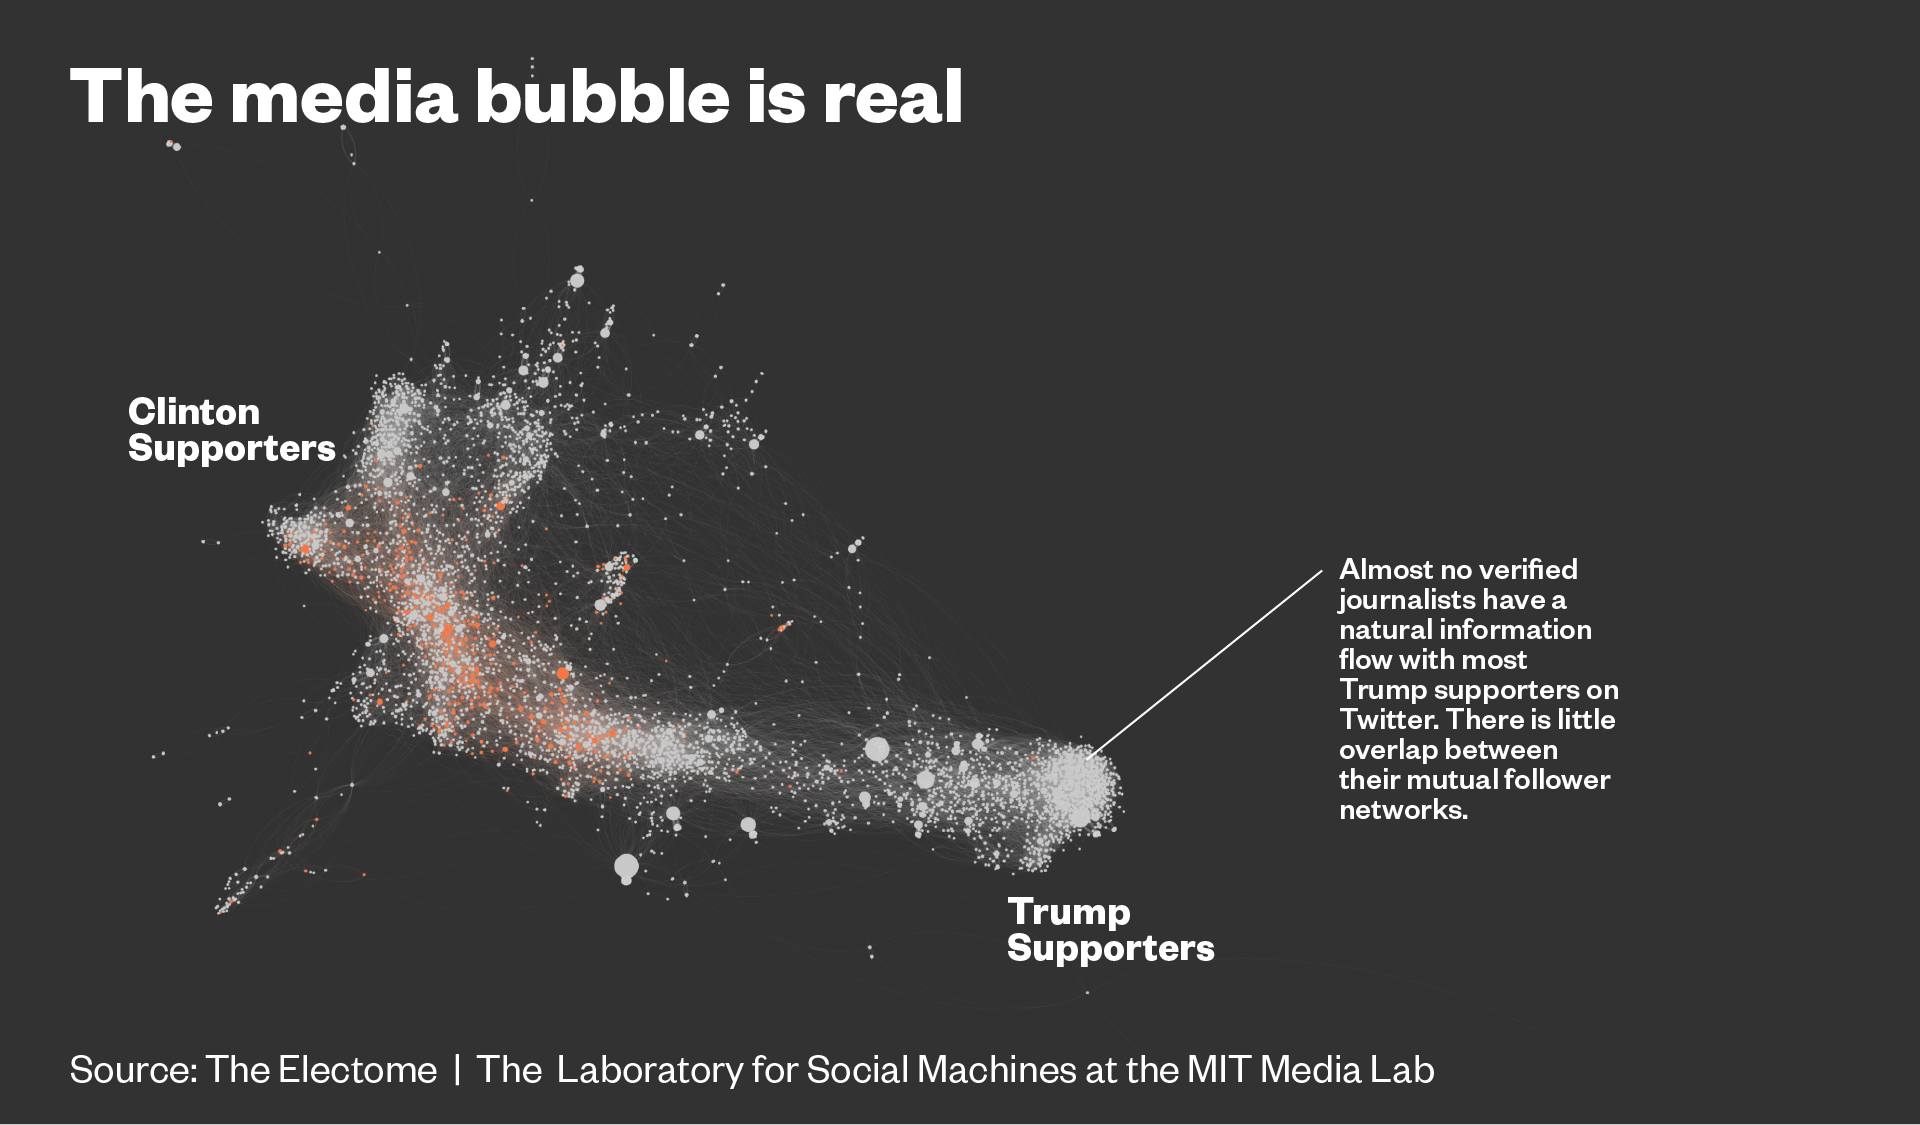
\includegraphics[width=\linewidth]{./images/election.png}
    \caption{Twitter follow networks for key influencers in the 2016 U.S. Presidential Election}
    \label{election}
\end{figure}

\section{Assessing Cluster Quality}
There are several methods for evaluating the quality of clusters. Leskovec et al. at Stanford performed an emperical comparision of several community detection algorithms, including the spectral-based graph partitioning method Local Spectral (similar to Spectral Bisection below), and the flow-based partitioning algorithm Metis+MQI (similar to Edge Betweenness below) \cite{Leskovec:2010:ECA:1772690.1772755}. They apply these methods to various data sets.
\par
The primary community score metric they use is conductance. Conductance measures cluster quality by looking at the ratio of edges in the community to the number of edges that leave that community. Formally, conductance is expressed as:

\begin{align}
    \phi(S) &= \frac{c_S}{min(Vol(S), Vol(V \setminus S))} \\
    c_S &= |{(u, v) : u \in S, v \notin S}| \\
    Vol(S) &= \sum_{u \in S}d(u)
\end{align}

where $S$ is the set of nodes in the community, $d(u)$ is the degree of node $u$. This captures both the connectedness of the community, as well as the connectedness of the community to the rest of the graph. The obejctive for a community detection algorithm is to minimize conductance. Conductance can also be taken for a partitioning of a graph with multiple cuts by taking the minimum conductance for any cut.
\par
The authors identify that there are two key criteria for assessing the quality of clusters, the number of edges within a cluster, and the number of edges that join that cluster with the rest of the graph. They group the remaining quality scores into two groups, those that depend on both of these criteria (multi-criterion scores), and those that depend on only one of these criteria (single criterion scores) \cite{Leskovec:2010:ECA:1772690.1772755}.
\par
It is evident that conductance is a multi-criterion score as is depends on edges within the community as well as edges that leave the community. There are several other multi-criterion scores including expansion, internal density, and cut ratio. Expansion is given as:

\begin{align}
    f(S) &= \frac{c_S}{n_S}
\end{align}

where $c_S$ is the number of edges on the boundary of set $S$, and $n_S$ is the number of nodes in $S$. Internal density is given as:

\begin{align}
    f(S) &= 1 - \frac{m_S}{n_S(n_S - 1)/2}
\end{align}

where $m_S$ is the number of edges in $S$. Finally, cut ratio is given as:

\begin{align}
    f(S) &= \frac{c_S}{n_S(n - n_S)}
\end{align}

where $n$ is the number of nodes in the entire graph. One key single cirterion score is modularity, which is given by:

\begin{align}
    f(S) &= \frac{1}{4m}(m_S - E(m_S))
\end{align}

where $E(m_S)$ is the expected number of edges in a random graph where the degrees of each node remain the same as the original community $S$. This measure is discussed more under Modularity.

\section{Algorithms}
Several algorithms have been introduced to mine communities from connection information. Several of these algorithms are discussed here, along with details of my reimplementation of these algorithms. Each of my implementations of these algorithms receives an iGraph graph object. The output is a VertexClustering object (and VertexDendrogram, if applicable) which is provided by iGraph and represents a clustering on a specific graph object. All of the code for these methods is writen in Python and provided by the GitHub repo:

\textit{https://github.com/jakecarlson1/community-finding}

    \subsection{Spectral Bisection}
    The spectral bisection method for detecting communities in graphs proposed by Pothen et al. involves using the eigenvectors of the Laplacian matrix for a graph to determine where to cut the graph \cite{doi:10.1137/0611030}. The Laplacian matrix for a graph is given by:

    \begin{align}
        L &= D - A
    \end{align}

    where $D$ is the diagonal matrix containing the degrees of each vertex, and $A$ is the adjacency matrix for the graph. Once this matrix is found, the goal is to cut the graph such that there are minimum edges running between the partitions, and the partitions are as close as possible to each other in terms of size. The graph can be divided by taking the median value $x$ of the eigenvector with the second smallest eigenvalue of the Laplacian matrix. This is known as the Fiedler vector, after Miroslav Fiedler who showed that the eigenvalue for this eigenvector represents the algebraic connectivity of the graph. This means that the second eigenvector for the Laplacian most efficiently divides the graph into two partitions. Because we need each vertex to be placed in either group 1 or group 2, it can be difficult to select a vector for dividing the graph that is parallel to the second eigenvector. Instead, we can look at the components of the eigenvector. This is why we look at the median value of the eigenvector and assign vertices to their groups based on the sign of their component of the eigenvector \cite{Newman2006.2}.
    \par
    Using this vector, the graph is then split into two sets, $A$ and $B$ where $A$ has verticies whose components are less than or equal to $x$, and $B$ has all vertices whose components are greater than $x$. If the difference in the sizes of these sets is greater than one, verticies whose components equal $x$ are arbitrarily reassigned to $B$ until the difference in the sizes of $A$ and $B$ is one.
    \par
    We then consider the set of edges who have one vertex in $A$ and another vertex in $B$. This is an edge separator of the graph, taken from the bipartite graph contained in $A$ and $B$. With this edge separator, it is possible to compute the minimum vertex cover of the bipartite graph contained in $A$ and $B$ by looking at the maximum matching of this bipartite graph. This cover is then used as the vertex separator to divide the graph into two parts.
    \par
    For my implementation, I build a the Laplacian matrix for the graph, and then use a spectral solver function to determine the optimal cut from the eigenvectors of the matrix. The vertices are partitioned into two sets as described above, and then the maximum bipartite matching function is used to find the set of vertices to split the graph on.

    \subsection{Edge Betweenness}
    In 2002, Girvan and Newman developed a new partitioning method by looking at the edges that are least central to communities. This development was motivated by shortcomings of a heirarchical clustering algorithm when applied to community detection. The issue Girvan and Newman found was that the heirarchical method would often take a vertex that shared a single edge with a community, and split this vertex into a community of its own. Girvan and Newman thought it was intuitive that a vertex that has only one edge should belong to the community that contains the vertex at the other end of that edge \cite{Girvan7821}.
    \par
    To account for this, Girvan and Newman developed a new method for partitioning a graph based on looking for edges that are the most "between" communities, rather than looking at those that are most central to the communities as heirarchical clustering does. Instead of iteratively adding the strongest edges to a set of verticies, the new method iteratively removes edges from the original graph. Girvan and Newman extend Freeman's betweenness centrality to determine the edges that are the most between communities.
    \par
    Freeman's betweenness centrality is based off of finding the shortest path connecting two nodes. More formally, the betweenness centrality for some vertex $k$ is the number of shortest paths between all other pairs of verticies $i$ and $j$ such that the shortest path between $i$ and $j$ contains $k$. Girvan and Newman generalize this to apply to edges, where the betweenness of an edge is defined as the number of shortest paths that run along that edge.
    \par
    Once the betweenness has been calculated for all edges in the graph, the edge with the highest betweenness is removed. The betweenness is then recalculated for the new graph, and the next edge with the highest betweenness is removed. This process repeats until there are no more edges in the graph.
    \par
    In my implementation of edge betweenness, I repeatedly remove the edge with the highes betweenness until no edges remain. This produces a sequence of edges. This sequence in reverse is the sequence of merges needed to build the graph, in order of minimum betweenness. This reversed sequence can be passed to the VertexDendrogram object to build a hierarchy of merges and a clustering object.

    \subsection{Modularity}
    Using modularity to detect communities in graphs was first proposed by Newman in 2006 \cite{Newman2006}. Newman identified that many community mining methods assume the network divides appropriately into subgroups, however, real-world social networks rarely behave this way. Instead, users can belong to several communities. In addition, typical graph partitioning algorithms are not suited well for community detection. These methods usually use minimum cut to divide the graph into subgroups. This is an intuitive method to apply, as it will minimize the number of edges running between the communities. However, you may need to constrain the size of the communities to prevent trivial solutions to dividing the network.
    \par
    For example, if the goal is to minimize edges between groups, the most straight-forward solution would be to create two groups, one of which is empty and one of which contains the rest of the network. This produces a count of edges between groups of zero. This trivial solution can be avoided by saying there needs to be at least $k$ nodes in each subgroup, but this requires determining this value ahead of time. Because of this, Newman was motivated to develop a new community detection method that is more applicable to real data.
    \par
    One goal Newman had was to eliminate the dependency on constraining the subgroup sizes as is required by other graph partitioning algorithms. This would avoid the problem of trivially dividing a network into two subgroups where one is empty and the other contains the rest of the graph. To achieve this, Newman introduces the modularity matrix. The modularity matrix is defined using the following equation for each element of the matrix \cite{Newman2006}:

    \begin{align}
        B_{ij} &= A_{ij} - E_{ij} \\
        E_{ij} &= \frac{k_ik_j}{2m}
    \end{align}

    Where $A_{ij}$ is the count of the edges between nodes $i$ and $j$, and $E_{ij}$ is the expected number of edges between the two nodes, given that $k_n$ is the degree of some node $n$ and $m$ is the total number of edges in the network. One important property of this matrix is that all of the rows and columns sum to zero, meaning it has an eigenvector (1, 1, 1,...) with an eigenvalue of zero. This is similar to the Laplacian Matrix from the Spectral Bisection Method. This matrix is then represented as a linear combination of normalized eigenvectors.
    \par
    The method for dividing the network into groups is borrowed from Spectral Partitioning. Newman repeatedly selects the largest, positive eigenvalue as the basis for dividing the network. The network is then divided based on the values in the eigenvector, where positive values are grouped together and negative values are grouped together. It can also be noted that the magnitude of these values indicate the strength of which an element belongs to a subgroup. Large values indicate an element belongs with a group, while values close to zero indicate the element may fall between the two groups.
    \par
    This process continues until there are no more positive eigenvalues for the modularity matrix. This allows the algorithm to stop once the network is indivisible, while also preventing the need for determining the size of the subgroups ahead of time.
    \par
    For my implementation, I first build the modularity matrix for the provided graph. Then, I pass this matrix and graph to the spectral solver used for the spectral bisection method, as these method use a similar process to partition the graph. There are two key differences when running this solver on the modularity matrix. The first is that we use the eigenvector with the largest eigenvalue, instead of the eigenvector with the second smallest eigenvalue. The second change is that, instead of using the median value for this eigenvector as the value to partition the nodes on, we set the value to 0 so that we are partitioning the graph based on the signs of the components of each vertex in the chosen eigenvector. Finally, we set the membership of each vertex so that the graph contains the clustering information.

    \subsection{Walktrap}
    In 2005, Pascal Pons and Matthieu Latapy introduced an entirely different method for finding community structure in networks. Their method, named Walktrap, is based on repeated random walks through the graph. The method is motivated by the intuition that a random walk through a densely connected region of the graph will tend to stay within that region \cite{10.1007/11569596_31}.
    \par
    This algorithm makes several assumptions about the data, including that the graph is connected, and that there is an edge between every node and itself. The algorithm begins by dividing the entire graph of $n$ verticies into $n$ communities of one node each. These communities are then iteratively merged based on a distance measure $r$.
    \par
    The authors define the distance between two communities, $r_{ij}$, based on the probability of encountering node $j$ given a random walk from $i$ of length $t$, $P^t_{ij}$. It is important to note that for a sufficiently high value of $t$, the probability of ariving at node $j$ approaches $\frac{k_j}{2m}$ where $k_j$ is the degree of node $j$ and $m$ is the number of edges in the graph. In other words, the probability of arriving at a node depends only on the degree of that node, and not the starting node for the random walk. This can be used to build the transition matrix $P$ for a graph. The transition matrix is given by:

    \begin{align}
        P &= D^{-1}A
    \end{align}

    The authors use the transition matrix to formally define the distance between two vertices by the equation:

    \begin{align}
        r_{ij} &= \sqrt{\sum^n_{k=1}{\frac{(P^t_{ik} - P^t_{jk})^2}{d(k)}}} = ||D^{-\frac{1}{2}}P^t_{i\bullet} - D^{-\frac{1}{2}}P^t_{j\bullet}||
    \end{align}

    This measure compares the probability of arriving at the same node $k$ when starting from both nodes $i$ and $j$. If the probabilities of arriving at $k$ are similar for all nodes in the graph, then the distance between $i$ and $j$ is small and they are likely part of the same community. Conversely, if the probabilities of arriving at $k$ differ for many entries in the probability lists, $i$ and $j$ are likely not in the same community.
    \par
    The transition matrix is leveraged to define the transition probability for a community of vertices as the normalized sum of the probability of arriving at any node in the community. The authors use the following equation to define the probability of arriving in a community:

    \begin{align}
        P^t_{Cj} = \frac{1}{|C|} \sum_{i \in C}P^t_{ij}
    \end{align}

    This then provides us with a way of determining the distance between two clusters by extending the distance equation above, but using the transition probability for communities rather than for vertices. This equation is:

    \begin{align}
        r_{C_1C_2} &= ||D^{-\frac{1}{2}}P^t_{C_1\bullet} - D^{-\frac{1}{2}}P^t_{C_2\bullet}||
    \end{align}

    This distance formula is used to choose the communities to merge. The authors base the merging of communities off of Ward's method, where each step selects communities to merge that minimize the mean of the squared distances between each vertex and the community it belongs to. We are trying to minimize the variation in this mean when merging two communities, which is given by:

    \begin{align}
        \Delta\sigma(C_1,C_2) &= \frac{1}{n}\frac{|C_1||C_2|}{|C_1| + |C_2|}r^2_{C_1C_2}
    \end{align}

    The authors note that their algorithm works well for short random walks fo $3 <= t <= 8$. The authors also advise decreasing $t$ if the graph is dense, and increasing $t$ if the graph is sparse. This is because the convergence speed of a random walk increases as the density of the graph increases \cite{10.1007/11569596_31}.
    \par
    Is should be noted that this is a closed form solution to a simulation of random walks through the graph. To better understand this algorithm, and to verify that the results are consistent between the two forms, I implement both the closed form and the simulated version of Walktrap.
    \par
    For the closed form implementation, I build the transition matrix by inverting the diagonal degree matrix and multiplying it by the adjacency matrix. I then raise the degree matrix to $-\frac{1}{2}$ and multiply this by the transition matrix to get the matrix that is ultimately used to calculate distances $T$. I then define a distance function that calculates the variance in the mean of the squared distances between two communities using the matrix $T$. I then pass the graph, the length of the random walk, and $T$ to a Walktrap solver.
    \par
    My Walktrap solver begins by generating a set of communities, each initialized with a 1-tuple containing a single vertex. I then build up a matrix of distances between vertices using the provided distance function. Since there can only be $|V| - 1$ merges, I also allocate space for future communities when building this distance matrix. All of these extra spaces are initialized with positive infinity to avoid selection when looking for the communities with the shortest distance.
    \par
    The solver then goes through the process of finding the two communities with the shortest distance, creating a new community for the joined set of vertices, calculating the distance to all of the other communities, setting all of the distances for the two merged communities to positive infinity to avoid selecting them again, and then calculating the modularity of the new partitioning using a built in iGraph modularity method. Once all of the merges have been performed, the maximum value in this array of modularities is used to select the optimal number of clusters for this method. I then build VertexDendrogram and VertexClustering objects that reference the initial graph parameter and contain all of the clustering information.
    \par
    The simulated implementation of this algorithm is very similar to closed form solution. The only difference is that I build the transition matrix by running $k$ random walks from each node in the graph, and normalize the number of times we arrived at each node by $k$. Each random walk uniformly chooses between edges of the current node, and then sets the neighbor on that edge as the current node. This happend $t$ times. I then pass this matrix to the same Walktrap solver used for the closed form solution. I also provide a distance fuction which only differs from the distance function for the closed form implementation by setting $t = 1$. This accounts for the fact that $t$ has already been used to calculate the transition matrix, and does not need to be multiplied by the probability vector of each vertex.

\section{Evaluation}
To examine the usefulness of these algorithms, I will use them to detect communities in Zachary's Karate Club data. I will compare the performance of my implementations against existing implementations in the iGraph package. This will provide insight into the correctness of my implementations as the results should be very similar when compared against iGraph. I will also evaluate the conductance of each partitioning to see which implementation produces the best conductance score (the minimum conductance).
\par
This data set represents the social network of a karate club. After the data was recorded, a dispute between two leaders of the group caused the club to split into two factions. The community detection algorithms should be able to determine where the karate club split into two groups.

    \subsection{Spectral Bisection}
    This method works well when the graph is easily separable into two distinct groups, however, it struggles when the graph is not easily separable \cite{Newman2004}. For the Karate Club data, spectral partitioning performs well. A side-by-side of the clusters determined by my implementation and the iGraph implementation is provided in Figure \ref{spec}.
    \par
    It is evident that my implementation produces the optimal community structure of the data set. The iGraph implementation produces more cuts that mine, due to different stopping criteria. My implementation stops after making one cut, while the iGraph implementation makes repeated cuts. It can be seen that by merging the red and blue communities from iGraph we will get the red community from my method, and by merging the green and yellow communities from iGraph, we will get my green community. The only node that this does not apply to is 8, which I say is in the red community and iGraph says it should be in my green community.
    \par
    The conductance of the partitioning produces by my implementation is $0.14$, while iGraph's implementation produced a clustering with a conductance of $0.25$. I believe this is happening because 8 is in different communities between my implementation and the iGraph implementation. The only other difference between implementations is that my implementation stops after making one cut, while iGraph makes cuts until there are no more valid cuts to make.

    \subsection{Edge Betweenness}
    Both my implementation of edge betweenness and the iGraph implementation perform well on this data set. The optimal number of communities is determined to be five for each method, but the clusters form much more distinguishable communities. Moreover, all nodes are clustered into the same groups between my implementation and the iGraph implementation. This verifies the accuracy of my implementation. The generated community structures are given in Figure \ref{eb}.
    \par
    The conductance of the partitioning produces by my implementation is $0.22$, while iGraph's implementation produced a clustering with a conductance of $0.22$. These value match indicating the two implementations produce results consistent with each other. This is also the best performing method for this data set, just short of walktrap.

    \subsection{Modularity}
    Modularity, similar to spectral bisection, also produces two communities. In the community structures, given in Figure \ref{mod}, vertex 8 is the only node classified differently. It is placed in the red group by my modularity implementation, even though it is placed in the what would be the opposite community by spectral bisection. Again, the iGraph implementation determines there are four communities in the data set. However, if you merge the red and blue clusters together, and the green and yellow clusters together, you get the same clustering as my implementation.
    \par
    The conductance of the partitioning produces by my implementation is $0.13$, while iGraph's implementation produced a clustering with a conductance of $0.23$. This is happening because conductance uses a one-versus-all methodology; it looks at the subset of nodes in the community versus all of the other nodes in the graph. If we merge the communities together as I stated above, we get the same conductance score as my partitioning of $0.13$.

    \subsection{Walktrap}
    The walktrap implementations perform the best on this data set. My closed form and simulated implementations produce the same clustering on this data set. The iGraph implementation also pulls out communities, but the optimal number of clusters is determined to be five. The detected communities are shown in Figure \ref{walktrap}. However, merging together the blue and red groups and the green, yellow, and pink groups produces the same clustering as my closed form and simulated solutions. The only difference is that vertex 13 is assigend to what is the green community in the first two community graphs in Figure \ref{walktrap} by iGraph, when it is determined to be in the opposite community by my implementation.
    \par
    When it comes to conductance, both of my implementations of walktrap produce a partitioning with the same conductance, $0.11$, however, the iGraph implementation produces a partitioning with a conductance of $0.25$. This slight difference is likely do to the difference in the community vertex 13 is assigned to. Again, if we calculate conductance on the merged communities as described above, we get a conductance of $0.12$. This is much closer to the conductance of my implementation. These conductance values also show that walktrap performs the best on this data set.

\section{Conclusion}
Here we saw the results of running several community detection methods agains Zachary's Karate Club. All of the methods shown were implemented for this and compared against implementations of the same algorithms by the iGraph package. It was found that the spectral partitioning methods of spectral bisection and modularity did not perform as well on this data set as some of the other methods, producing communities that were not clearly separated and had a higher conductance. Perhaps the performance of these implementations could be improved if they allowed multiple cuts of the data.
\par
The edge betweenness method produced good results on this data set, even though it overestimated the number of communities. The smaller communities could be merged with a heuristic to form the expected community structure. The walktrap method performed the best on this data set. The closed form and simulated implementations produce results that are almost identical to each other. Again, the iGraph implementation determines there are more communities than my methods found, but the cuts occur in similar locations and the overall conductance is the same as my methods.

\newpage
\bibliography{sources}
\bibliographystyle{plain}

\newpage

\begin{figure}[h]
    \begin{minipage}{0.48\textwidth}
    \colorbox{gray}{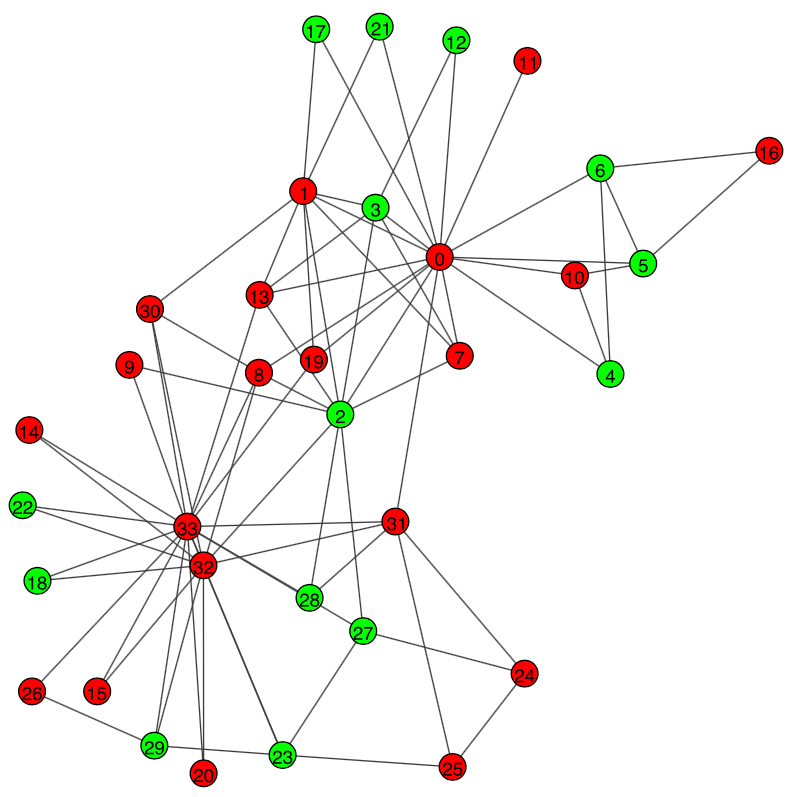
\includegraphics[width=\linewidth]{./images/mod-j.png}}
    \end{minipage}
    \hspace{\fill}
    \begin{minipage}{0.48\textwidth}
    \colorbox{gray}{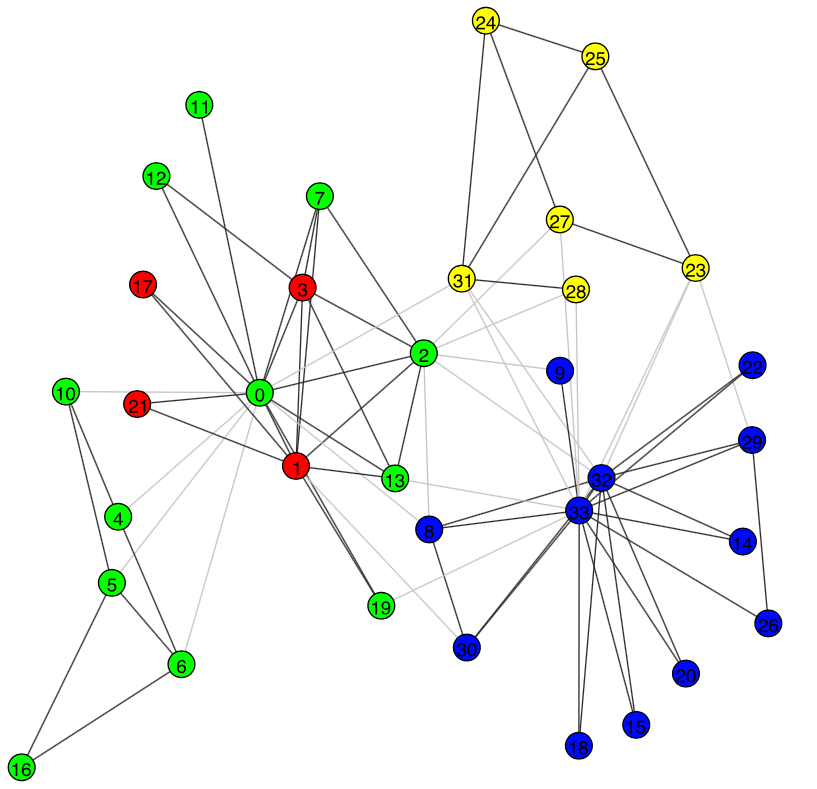
\includegraphics[width=\linewidth]{./images/mod-i.png}}
    \end{minipage}

    \caption{Result of modularity method on Karate Club. left: my implementation, right: iGraph implementation}
    \label{mod}
\end{figure}

\begin{figure}[h]
    \begin{minipage}{0.48\textwidth}
    \colorbox{gray}{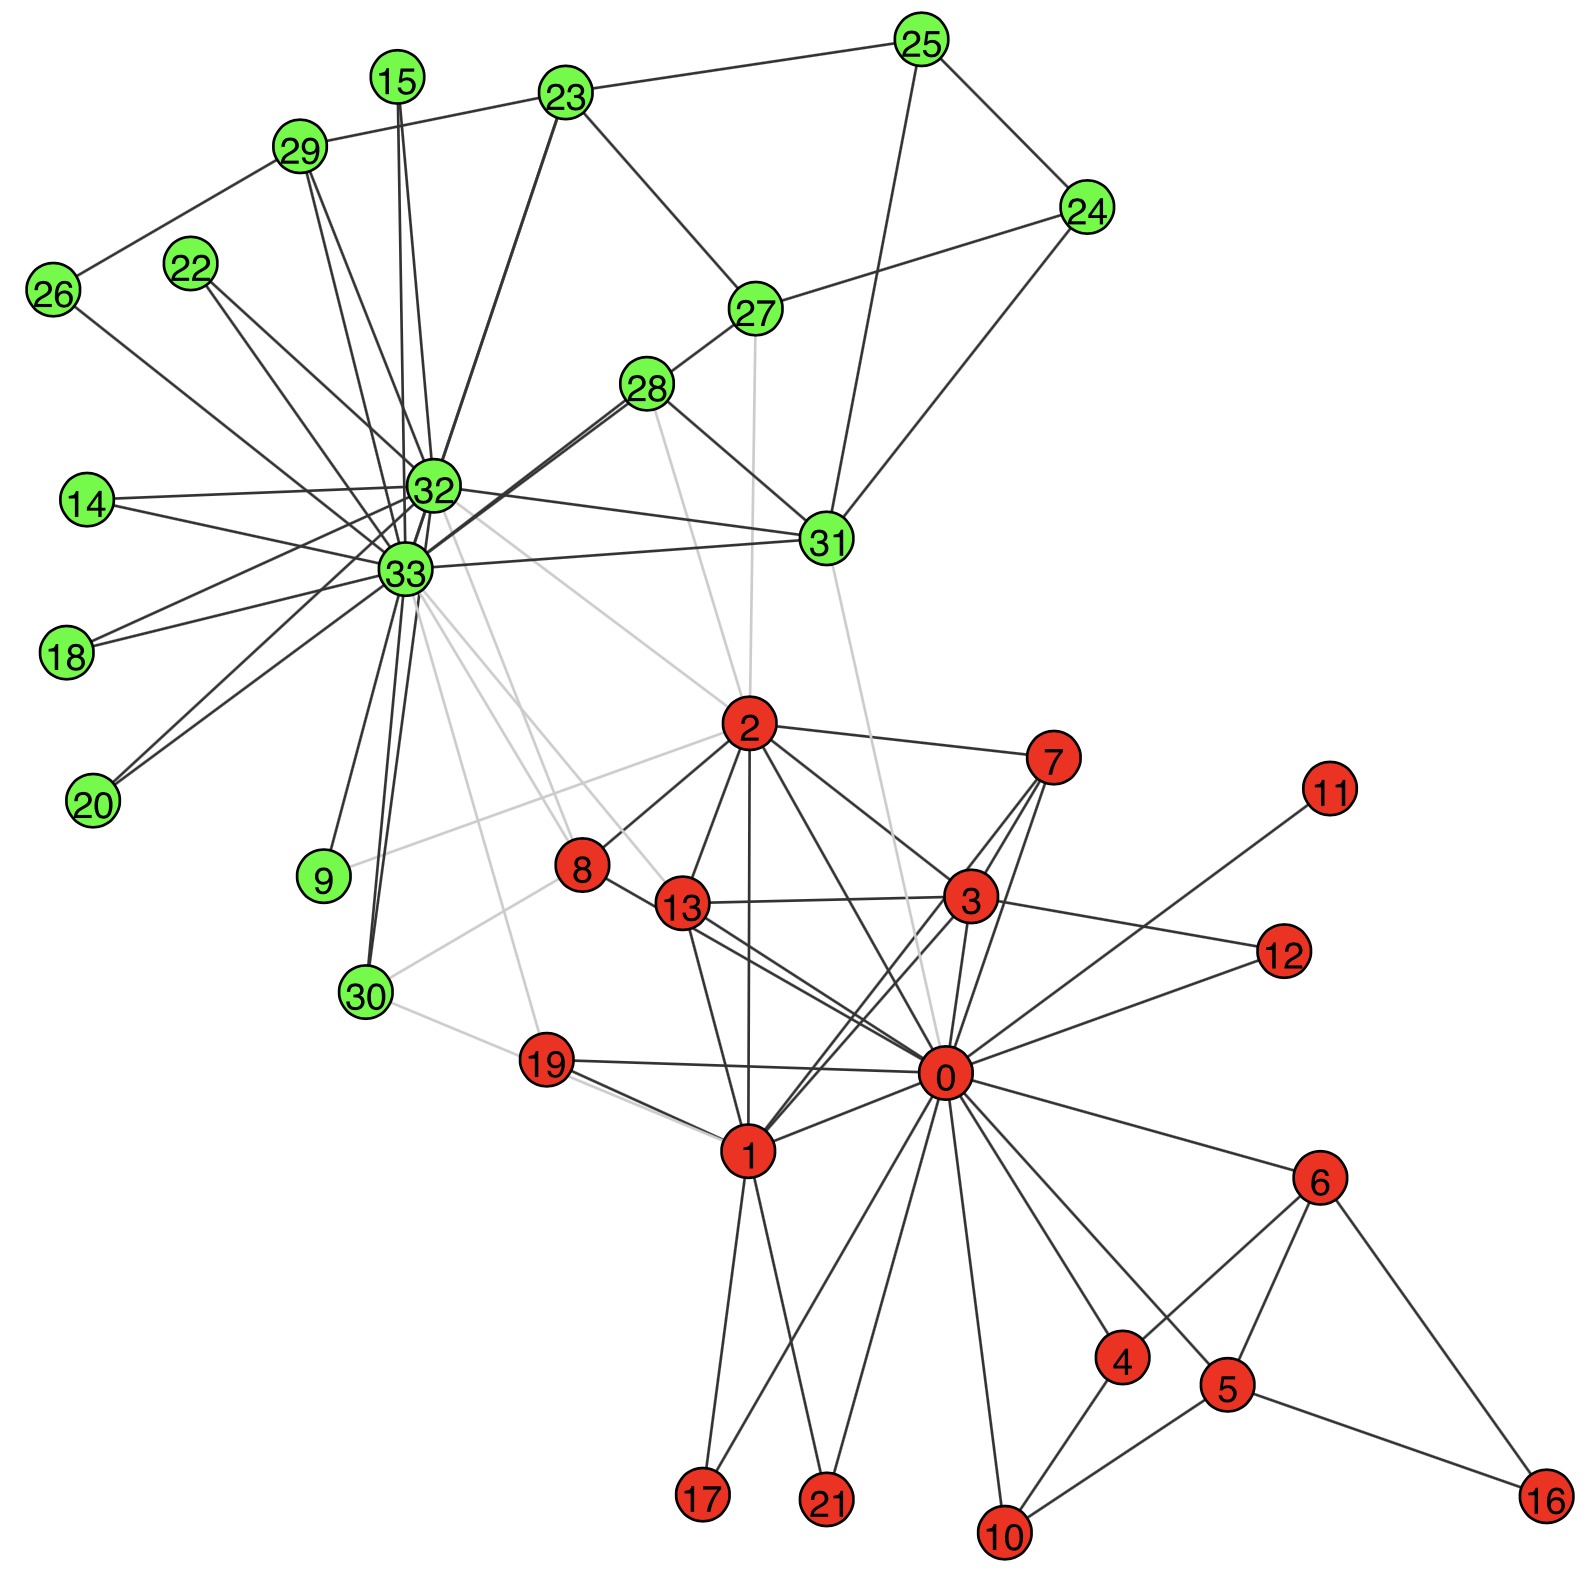
\includegraphics[width=\linewidth]{./images/spec-j.png}}
    \end{minipage}
    \hspace{\fill}
    \begin{minipage}{0.48\textwidth}
    \colorbox{gray}{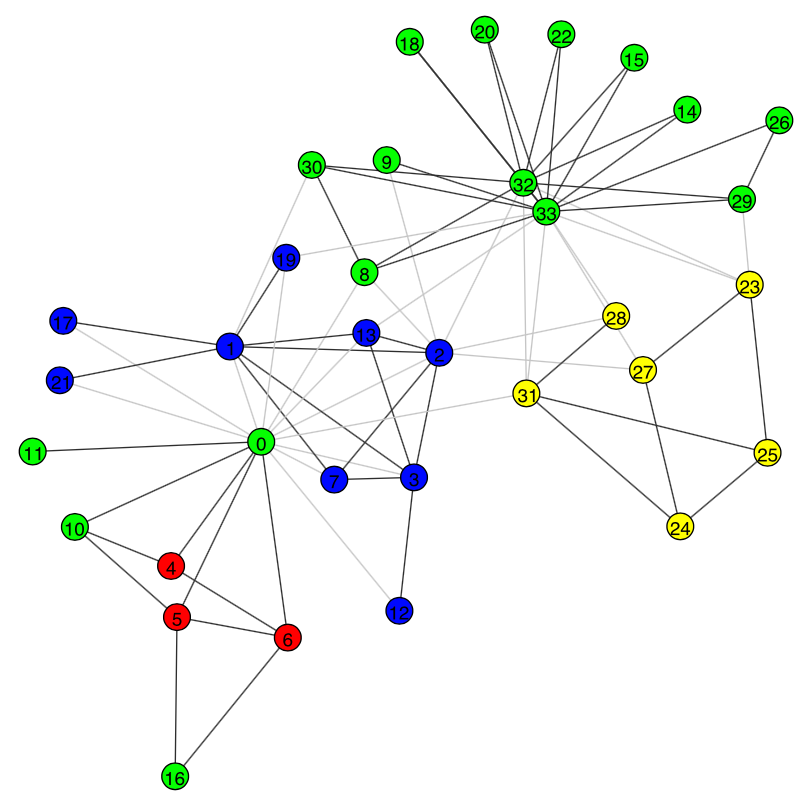
\includegraphics[width=\linewidth]{./images/spec-i.png}}
    \end{minipage}

    \caption{Result of spectral bisection method on Karate Club. left: my implementation, right: iGraph implementation}
    \label{spec}
\end{figure}

\begin{figure}[h]
    \begin{minipage}{0.48\textwidth}
    \colorbox{gray}{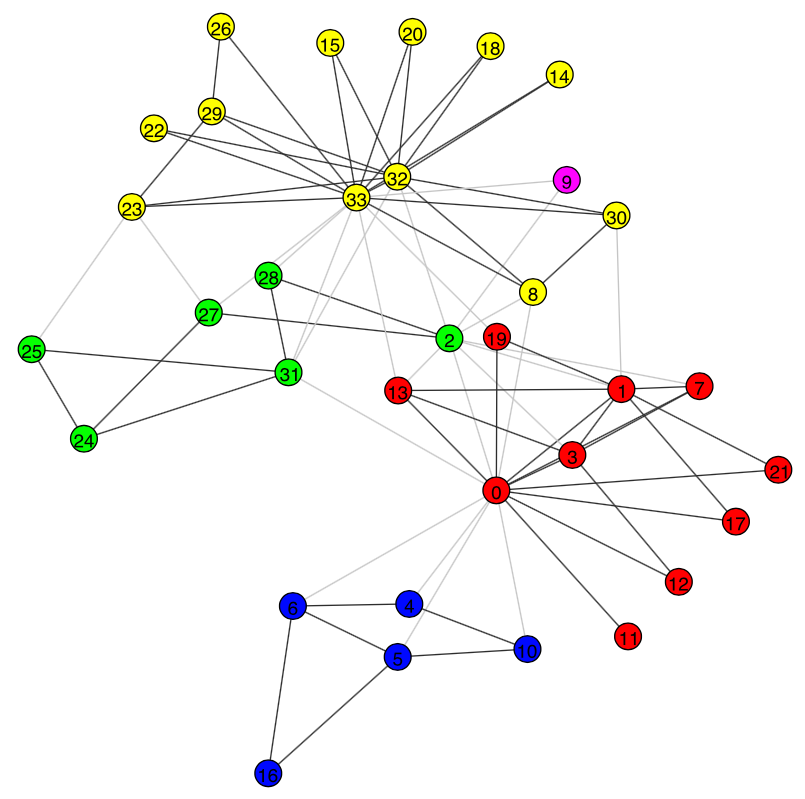
\includegraphics[width=\linewidth]{./images/eb-j.png}}
    \end{minipage}
    \hspace{\fill}
    \begin{minipage}{0.48\textwidth}
    \colorbox{gray}{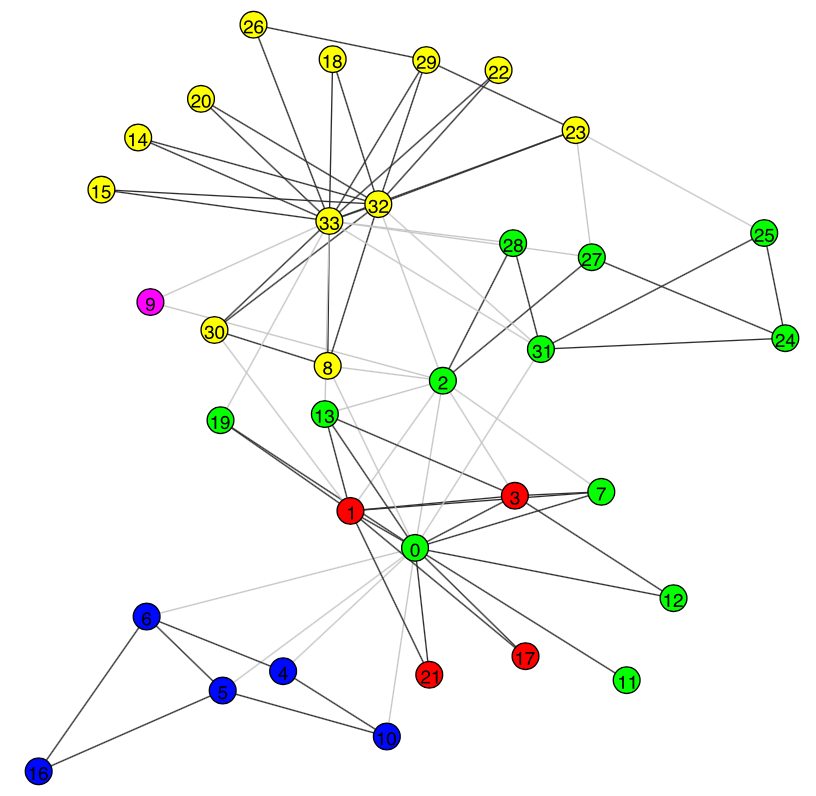
\includegraphics[width=\linewidth]{./images/eb-i.png}}
    \end{minipage}

    \caption{Result of edge betweenness method on Karate Club. left: my implementation, right: iGraph implementation}
    \label{eb}
\end{figure}

\begin{figure}[h]
    \begin{minipage}{0.3\textwidth}
    \colorbox{gray}{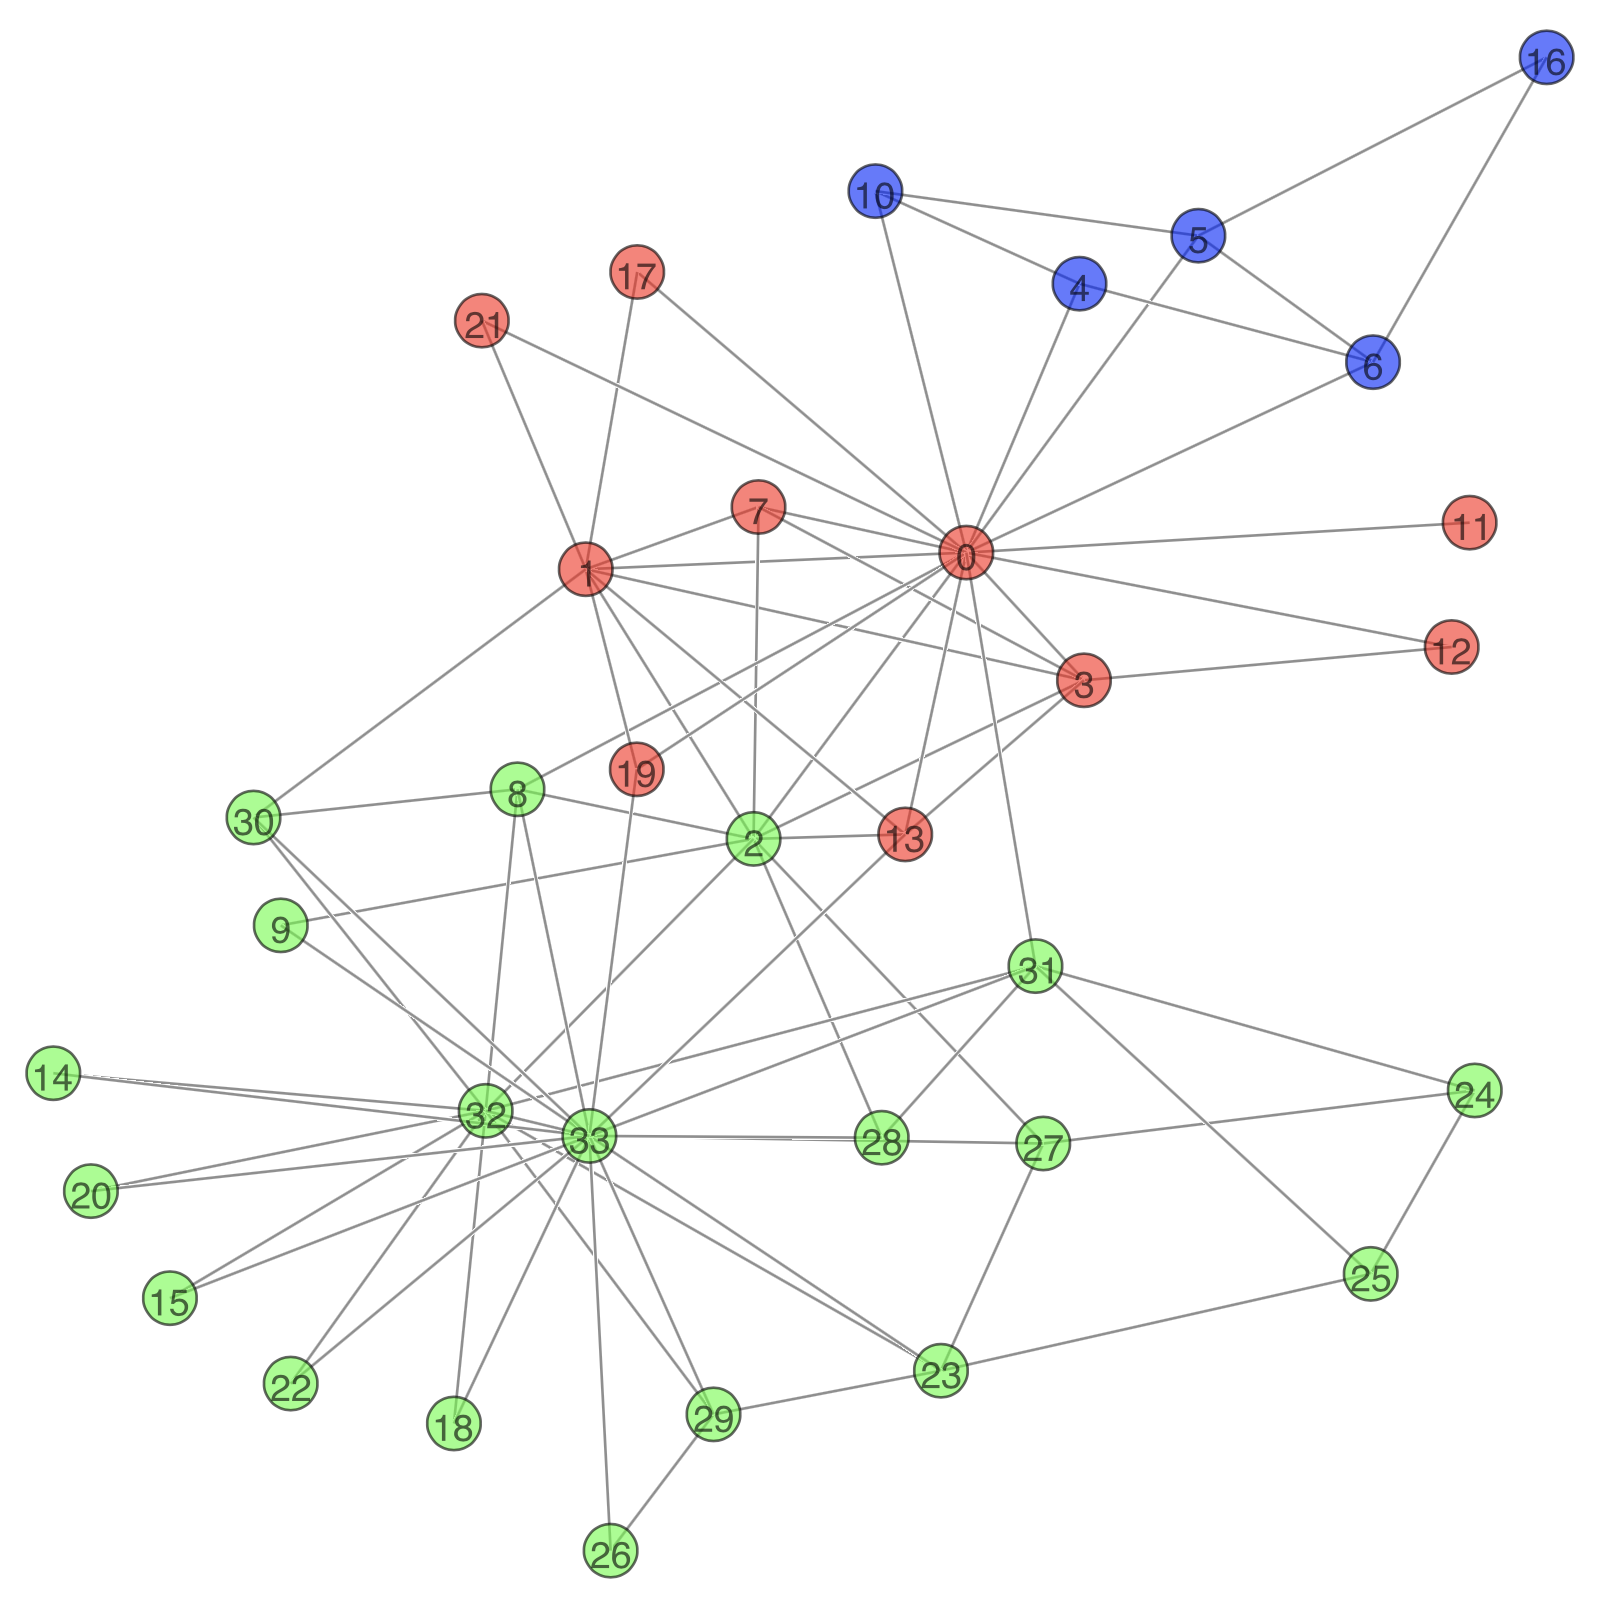
\includegraphics[width=\linewidth]{./images/walktrap-cf.png}}
    \end{minipage}
    \hspace{\fill}
    \begin{minipage}{0.3\textwidth}
    \colorbox{gray}{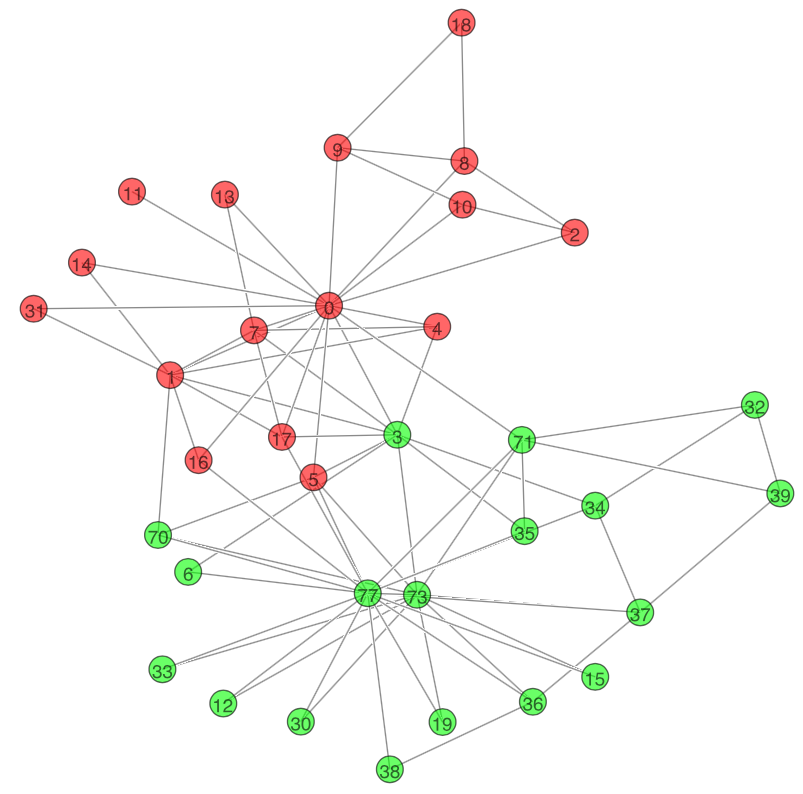
\includegraphics[width=\linewidth]{./images/walktrap-sim.png}}
    \end{minipage}
    \hspace{\fill}
    \begin{minipage}{0.3\textwidth}
    \colorbox{gray}{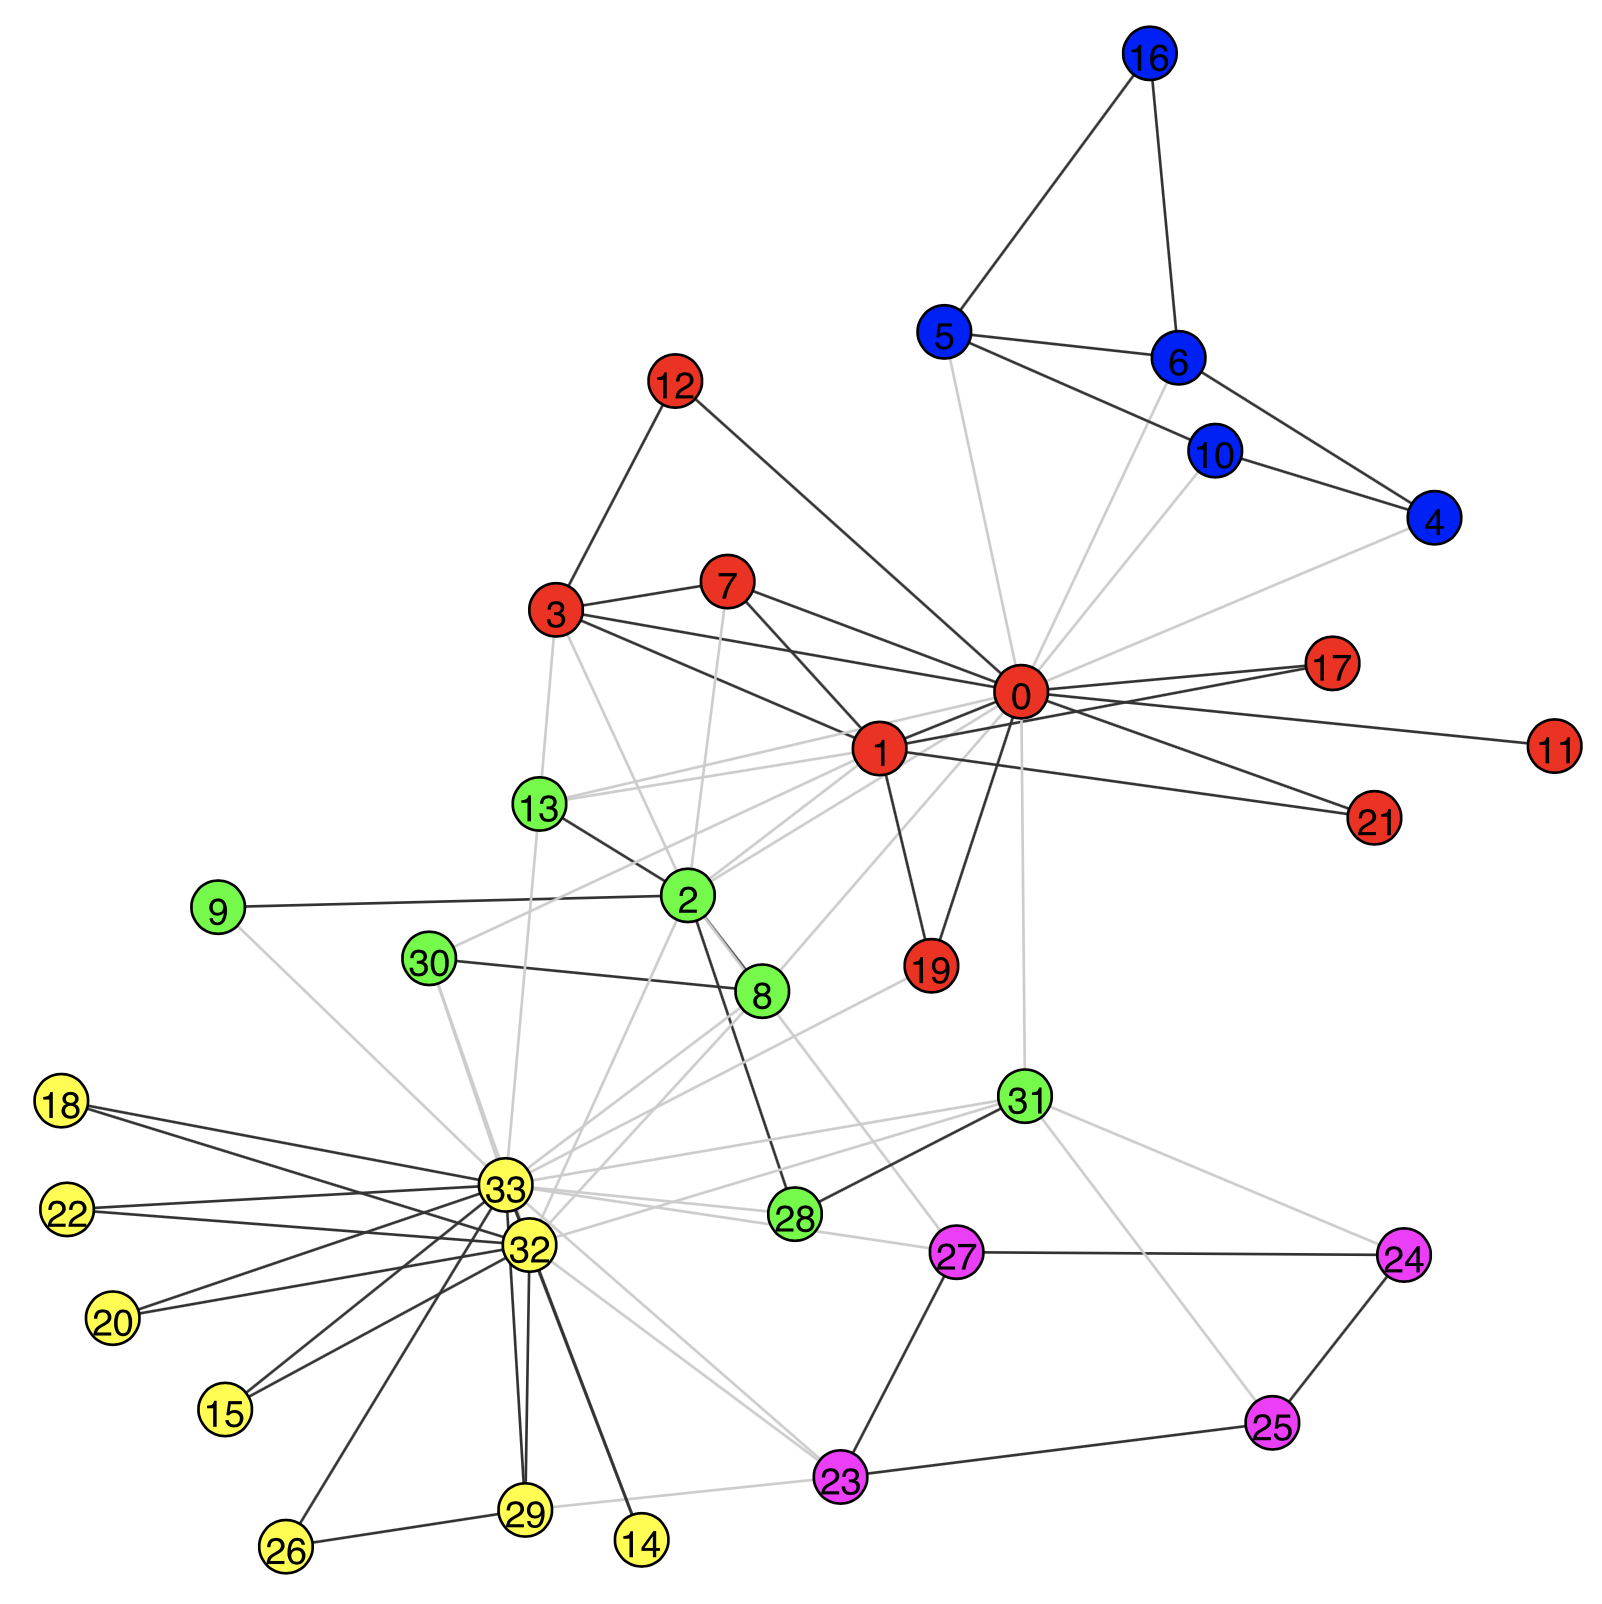
\includegraphics[width=\linewidth]{./images/walktrap-i.png}}
    \end{minipage}

    \caption{Result of walktrap method on Karate Club. left: my closed form implementation, center: my simulated implementation, right: iGraph implementation}
    \label{walktrap}
\end{figure}

\end{document}
